\subsection*{Global Sensor Networks}
\label{sec:gsn}

GSN~(Global Sensor Networks)~\cite{gsn, gsn0, gsn2} is a system targeting the construction of global sensing
infrastructure. Its aim is to make the publication and access to sensor network data as simple, powerful and flexible as
accessing Web documents. In its model, single sensors or entire sensor networks are connected to their sinks, which are
in turn connected to the Internet, that make their data available through a common interface. 
\begin{figure}[b]
	\centering
	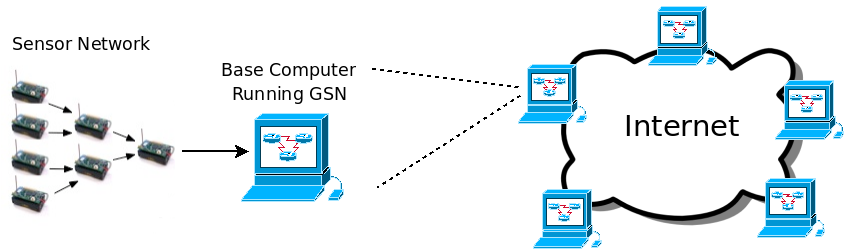
\includegraphics[scale=0.5]{img/mygsn.png}
	\caption{GSN architecture.}
	\label{fig:gsn-node}
\end{figure}



The basic abstraction provided by GSN is called \textit{virtual sensor}. These abstract from the actual implementation details and model
sensor data as temporal streams of relational data. They can also represents \emph{derived views}, which contain
composite information obtained from the processing of many data sources.
This allows to use a common abstraction, representing in unified way data coming from
various sensor types or derived from different raw sensor data. The streams of data, generated by the virtual sensors,
are published through a peer-to-peer directory. Each virtual sensor can be equipped with a set of key-value pairs,
describing its properties. Applications can select the subset of published data their are interested in based on their 
attributes, and access them by the mean of a standard access interface. 

Queries are expressed in a declarative way through
an SQL-based language. A mapping from virtual sensors to actual physical nodes is done by the mean of \emph{GSN
containers}, the actual building blocks of the GSN infrastructure. These containers cooperate as peers in a decentralized
system, they communicate through standard Internet protocols. Figure~\ref{fig:gsn-node} shows the architecture of a
the GSN infrastructure. Several sensor networks are connected through GSN. Every sensor network has a \emph{sink} node,
which collects all the readings from the nodes and has a connection to the outside. The sink communicates to a computer
running an instance of GSN, that represents the entry point for the computing infrastructure. Several machines are
connected through the Internet and represent the backbone onto which the actual computation takes place.

One of the main components is the \emph{Virtual Sensor Manager} (VSM), which is responsible of the access to the local virtual
sensors. Data to and from the VSM passes through the storage layer, which is in charge of managing persistent storage of
sensor data. The other important component of the GSN container is the \emph{Query Manager} (QM). This implements the query
processor in charge of executing the relational queries. The implementation of the GSN containers is done in Java, and to enable a new
class of sensors to be usable within GSN, all that is needed is a Java-based wrapper implementation.

\paragraph{Considerations}The architectural model proposed by GSN, with several sensor networks being the input sources for a backbone processing
infrastructure connected through the Internet is the same as the one I envision for DISSP. Sensor networks are designed
to reliably collect the sensor data, dealing with issues like networking, security and power efficiency. Once the data
is collected, it can be passed on to a higher level infrastructure to be processed. My work is focused on this second
level: on how to reliably process the data over a number of geographically distributed computing sites. 
GSN does not provide any sophisticated \emph{fault-tolerance} mechanism, if a node crashes, for instance, all the
resources associated with it disappear from the computation. Investigating new strategies for better fault-tolerance in
such a system is one of the objectives of my research.
